\documentclass[a4paper, 10pt, twoside]{article}

\usepackage[top=1in, bottom=1in, left=1in, right=1in]{geometry}
\usepackage[utf8]{inputenc}
\usepackage[spanish, es-ucroman, es-noquoting, activeacute]{babel}
\usepackage{setspace}
\usepackage{fancyhdr}
\usepackage{lastpage}
\usepackage{amsmath}
\usepackage{amsfonts}
\usepackage{amsthm}
\usepackage{algpseudocode}
\usepackage[]{algorithm2e}
\usepackage{verbatim}
\usepackage{fancyvrb}
\usepackage{graphicx}
\usepackage{float}
\usepackage{enumitem} % Provee macro \setlist
\usepackage{tabularx}
\usepackage{multirow}
\usepackage{hyperref}
\usepackage{lscape}
\usepackage{xspace}
\usepackage{qtree}
\usepackage[toc, page]{appendix}


%%%%%%%%%% Constantes - Inicio %%%%%%%%%%
\newcommand{\titulo}{Trabajo Práctico 1}
\newcommand{\materia}{Redes Neuronales}
\newcommand{\integrantes}{Barijhoff - Ishikame - Russo}
\newcommand{\cuatrimestre}{Segundo Cuatrimestre de 2016}
%%%%%%%%%% Constantes - Fin %%%%%%%%%%

%%%%%%%%%% Configuración de Fancyhdr - Inicio %%%%%%%%%%
\pagestyle{fancy}
\thispagestyle{fancy}
\lhead{\titulo\ · \materia}
\rhead{\integrantes}
\renewcommand{\footrulewidth}{0.4pt}
\cfoot{\thepage /\pageref{LastPage}}

\fancypagestyle{caratula} {
   \fancyhf{}
   \cfoot{\thepage /\pageref{LastPage}}
   \renewcommand{\headrulewidth}{0pt}
   \renewcommand{\footrulewidth}{0pt}
}
%%%%%%%%%% Configuración de Fancyhdr - Fin %%%%%%%%%%


%%%%%%%%%% Miscelánea - Inicio %%%%%%%%%%
% Evita que el documento se estire verticalmente para ocupar el espacio vacío
% en cada página.
\raggedbottom

% Separación entre párrafos.
\setlength{\parskip}{0.5em}

% Separación entre elementos de listas.
\setlist{itemsep=0.5em}

% Asigna la traducción de la palabra 'Appendices'.
\renewcommand{\appendixtocname}{Apéndices}
\renewcommand{\appendixpagename}{Apéndices}

\newcommand{\diagrama}[1]{
  \begin{center}
    \includegraphics[width=16cm]{#1}
  \end{center}
}

\newcommand{\diagramadeancho}[2]{
  \begin{center}
    \includegraphics[width=#1]{#2}
  \end{center}
}

\newcommand{\riesgo}[7]{
  \underline{Riesgo {#1}:}
  \begin{itemize}   
    \item \textbf{Descripción:} {#2}
    \item \textbf{Probablidad:} {#3}
    \item \textbf{Impacto:} {#4}
    \item \textbf{Exposición:} {#5}
    \item \textbf{Mitigación:} {#6}
    \item \textbf{Plan de contingencia:} {#7}
  \end{itemize}
}

\newcommand{\escenario}[7] {
  \textit{{#1}}
  \begin{itemize}
    \item \textbf{Fuente:} {#2}
    \item \textbf{Estímulo:} {#3}
    \item \textbf{Entorno:} {#4}
    \item \textbf{Artefacto:} {#5}
    \item \textbf{Respuesta:} {#6}
    \item \textbf{Medición:} {#7}
  \end{itemize}
}

%%%%%%%%%% Miscelánea - Fin %%%%%%%%%%

\begin{document}


%%%%%%%%%%%%%%%%%%%%%%%%%%%%%%%%%%%%%%%%%%%%%%%%%%%%%%%%%%%%%%%%%%%%%%%%%%%%%%%
%% Carátula                                                                  %%
%%%%%%%%%%%%%%%%%%%%%%%%%%%%%%%%%%%%%%%%%%%%%%%%%%%%%%%%%%%%%%%%%%%%%%%%%%%%%%%


\thispagestyle{caratula}

\begin{center}


\includegraphics[height=2cm]{DC.png} 
\hfill

\includegraphics[height=2cm]{UBA.jpg} 

\vspace{2cm}

Departamento de Computación,\\
Facultad de Ciencias Exactas y Naturales,\\
Universidad de Buenos Aires

\vspace{4cm}

\begin{Huge}
\titulo
\end{Huge}

\vspace{0.5cm}

\begin{Large}
\materia
\end{Large}

\vspace{1cm}

\cuatrimestre

\vspace{4cm}

\begin{tabular}{|c|c|c|}
\hline
Apellido y Nombre & LU & E-mail\\
\hline
Barijhoff, Hernan           & 338/13 & hernanfb@live.com.ar \\
Ishikame, Emiliano               & 861/11 & emilianoishikame@yahoo.com.ar \\
Russo, Christian              & 679/10 & christian.russo8@gmail.com\\
\hline
\end{tabular}

\end{center}

\newpage

\tableofcontents

\newpage


%%%%%%%%%%%%%%%%%%%%%%%%%%%%%%%%%%%%%%%%%%%%%%%%%%%%%%%%%%%%%%%%%%%%%%%%%%%%%%%
%% Introducción                                                              %%
%%%%%%%%%%%%%%%%%%%%%%%%%%%%%%%%%%%%%%%%%%%%%%%%%%%%%%%%%%%%%%%%%%%%%%%%%%%%%%%

\section{Introduccion y Teoria}
\subsection{Introduccion}
En el presente trabajo utilizaremos redes neuronales artificiales entrenadas con retropropagacion de errores (backpropagation) para modelar dos problemas distintos. La idea sera entrenar la red con informacion contenida en dos bases de datos.

El primer problema consiste en dada unas muestras de tumores de mamas, poder calificar si un tumor corresponde o no con tumores \textbf{malignos} o \textbf{benignos}.

El segundo problema dada una muestra con ciertos atributos de edificios, tales como superficie total u oritancion, podremos precedir la \textbf{cantidad de energia necesaria para calefaccionar y refrigerar los edificios}.

Se espera entonces que utilizando lo que vimos en la materia podamos desarrollar redes que resuelvan correctamente ambos problemas. 

Adicionalmente se espera hacer un analisis y experimentacion del funcionamiento de un perceptron multicapa con retropropagacion de errores.

\subsection{Introduccion Teorica}
La idea principal del perceptron multicapa es utilizar el paradigma de aprendizaje supervisado con un algoritmo de correccion de errores. Es una red neuronal artificial formada por multiples capas, esto le permite resolver problemas que no son linealmente separables, lo cual es la principal limitación del perceptron simple.

\begin{center}
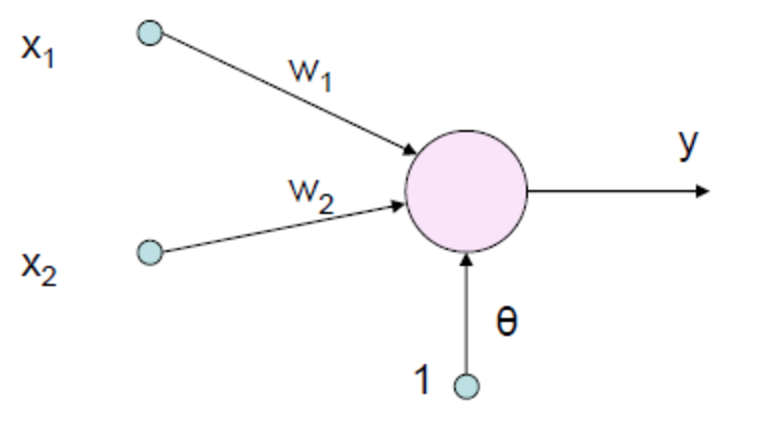
\includegraphics[width=0.25\textwidth]{img/psimple}
\end{center}

El aprendizaje supervisado se basa en un entrenamiento en el cual se provee al sistema con informacion de las entradas y de igual forma se proveen las salidas esperadas para cada entrada en particular.

Intuitivamente, el perceptron multicapa permite aproximar funciones, categorizar y encontrar patrones.

\begin{center}
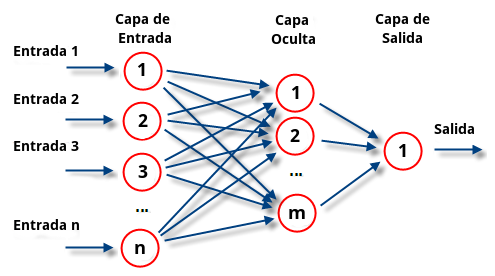
\includegraphics{img/pmulticapa}
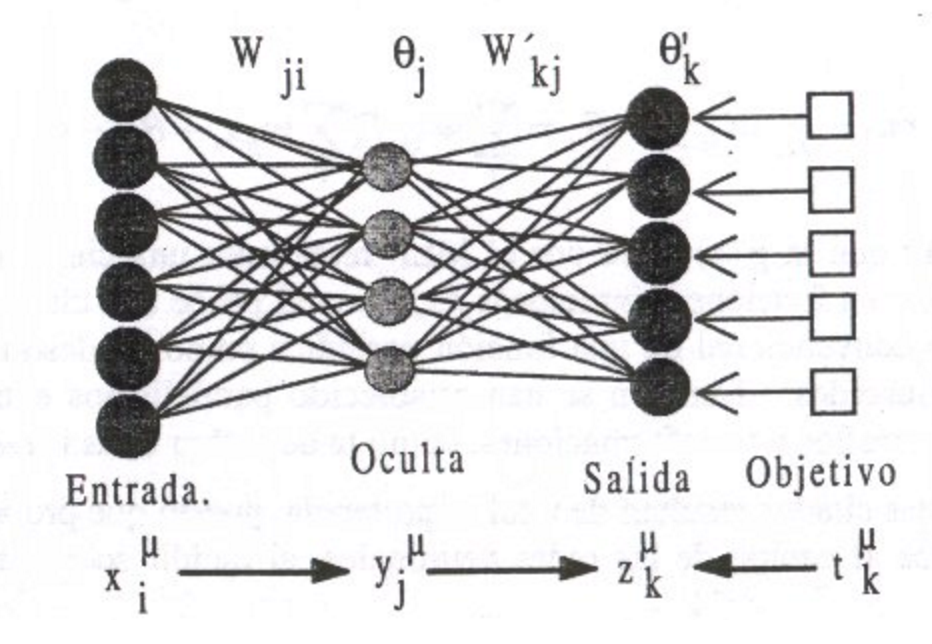
\includegraphics[width=0.35\textwidth]{img/pmulticapa2}
\end{center}

Las neuronas de la capa oculta usan como regla de propagacion la suma ponderada de las entradas con los pesos sinápticos $w_{ij}$ y sobre esa suma ponderada se aplica una funcion de transferencia de tipo sigmoide, que es acotada en respuesta.

\newpage
Grafico de funcion sigmoide:

\begin{center}
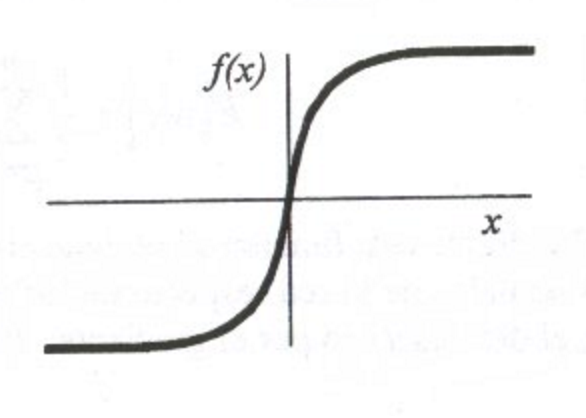
\includegraphics[width=0.30\textwidth]{img/sigmoide}
\end{center}

Sobre el aprendizaje, para este se suele usar en este tipo de redes recibe el nombre de backpropagation. Como funcion de coste global, se usa el error cuadratico medio. Es decir, que dado un par ($x_k$, $d_k$) correspondiente a la entrada k de los datos de entrenamiento y salida deseada asociada se calcula la cantidad.

Por otro lado, las capas pueden clasificarse en tres tipos:

\begin{enumerate}
\item \textbf{Capa de entrada:} Constituida por aquellas neuronas que introducen los patrones de entrada en la red. 
\item \textbf{Capas ocultas:} Formada por aquellas neuronas cuyas entradas provienen de capas anteriores y cuyas salidas pasan a neuronas de capas posteriores.
\item \textbf{Capa de salida:} Neuronas cuyos valores de salida se corresponden con las salidas de toda la red.
\end{enumerate}


En general la estructura de una neurona se puede representar de la siguiente manera:

\begin{center}
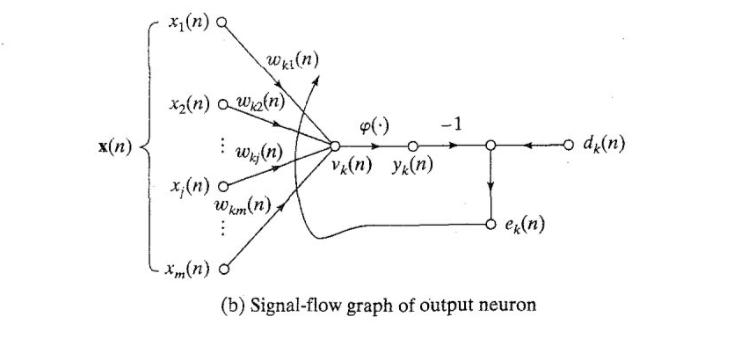
\includegraphics[width=0.6\textwidth]{img/neurona}
\end{center}

Podemos observar como los elementos mas importantes al vector de entrada de la neurona $(x_1,...,x_m)$, a los pesos correspondientes como $w_{ij}$, a la funcion de activacio y al elemento de salida. A partir de esta estructura basica la neurona puede mapear las entradas para obtener a la salida una respuesta deseada que pudiera pertenecer a alguna funcion a de terminar.


La funcion de activacion trata de simular el mecanismo que realiza el sistema de neuronas en el cerebro, que se basa en la exitacion de las neuronas hasta un cierto punto en el cual se pasa un umbral en el que dicha neurona dispara la informacion que le corresponde. Entre las diferentes funciones de activacion podemos encontrar la sigmoide.


Por otro lado el perceptron cuenta con un coeficiente de entrenamiento que indica que tanto varian los pesos entre iteracion e iteracion, por lo cual indica que tan lento o rapido la red se entrena.
\section{Ejercicio: Cancer de mamas}
\subsection{Explicacion}
Los datos son resultado de un examen que se realizan para diagnosticar cancer de mamas. Para cada paciente contamos con 10 caracteristicas de las imagenes de las celulas, entre estas caracteristicas contamos con diagnostico, radio, perimetro, textura, area, suavidad, etc. 

Cada una de estas entradas corrresponde a los datos de distintos pacientes, es importante remarcar que se cuenta con el atributo del diagnostico final quen indica si un tumor es benigno o maligno (0 y 1 respectivamente).

Sobre este primer dataset se buscara entrenar una red neuronal para poder predecir, dado un nuevo paciente con sus datos, si su estado sera el de tener cancer o no.

Este tipo de problemas se denomina un \textbf{problema de clasificacion}

\subsection{Resultados y analisis}
\subsection{Conclusiones}
\subsection{Codigo}
\section{Ejercicio: Eficiencia energetica}
\subsection{Explicacion}

En el siguiente problema contamos con los datos sobre la carga energetica para calefaccionar y refrigerar edificios en funcion de ciertas caractersisticas de los mismos.

El analisis se realizo tomando en cuenta edificios de diversas caracteristifcas, que difieren con respecto a la superficie y distribucion de las areas de reflejo, la orientacioon, etc.

Para cada edificio contamos con area de la superficie total, area de las paredes, area del techo, orientacion, area de reflejo total, etc.

Es importante remarcar que tambien contamos, para cada edifico del dataset, la cantidad de energio necersaria para realizar una calefaccion y refrigeracion adecuada.

Sobre este segundo dataset se buscara entrenar una red neuronal para poder aproximar la funcion que determina la cantidad de energia necesaria para
la calefaccion y refrigeracion de un edificio en funcion de los parametros de entrada. Es decir, es un problema de regresion.



\subsection{Resultados y analisis}
\subsection{Conclusiones}
\subsection{Codigo}
\section{Entregable}
\subsection{Contenido del entregable}
Lorem ipsum dolor sit amet, consectetur adipisicing elit, sed do eiusmod
tempor incididunt ut labore et dolore magna aliqua. Ut enim ad minim veniam,
quis nostrud exercitation ullamco laboris nisi ut aliquip ex ea commodo
consequat. Duis aute irure dolor in reprehenderit in voluptate velit esse
cillum dolore eu fugiat nulla pariatur. Excepteur sint occaecat cupidatat non
proident, sunt in culpa qui officia deserunt mollit anim id est laborum.

\subsection{Modo de ejecución}


\subsubsection{Ejercicio 1}


La manera de ejecutar el programa dado es la siguiente:

En caso de querer entrenar la red sera:

\begin{verbatim}
$ python main.py < archivo_entrada > < archivo_red_salida > -train < lrate > 
                                                   < max_epochs > < method >    
\end{verbatim}

Donde:

\begin{enumerate}
\item archivo\_entrada: archivo de dataset.
\item archivo\_red\_salida: archivo donde se guardara la red.
\item lrate: Coeficiente de aprendizaje.
\item max\_epochs: Maxima cantidad de epocas permitidas.
\item method: 
\begin{enumerate}
\item -s: Sanger
\item -o: Oja
\end{enumerate}
\end{enumerate}

Por ejemplo: 

Si queremos ejecutar el ejercicio 1 entrenandolo con el dataset \textbf{tp2\_training\_dataset.csv}, guardando la red en el archivo 
\textbf{red} con un learning\_rate de \textbf{0.01}, con un espacio de salida de \textbf{3}, con una cantidad maxima de epocas de \textbf{10000} y con el modo \textbf{Sanger} seria:

\begin{verbatim}
$ python main.py tp2_training.dataset.csv  red -train 0.01 10000 -s
\end{verbatim}

En caso de querer cargar una red ya guardada seria:

\begin{verbatim}
$ python main.py < archivo_entrada > < nombre_red_in > -load
\end{verbatim}

Donde:

\begin{enumerate}
\item archivo\_entrada: archivo de dataset.
\item nombre\_red\_in: nombre de la red a cargar.
\end{enumerate}

Por ejemplo, si queremos cargar la red llamada \textbf{red} con el dataset \textbf{tp2\_training\_dataset.csv} seria:

\begin{verbatim}
$  python main.py tp2_training_dataset.csv red -load
\end{verbatim}

\subsubsection{Ejercicio 2}

La manera de ejecutar el programa dado es la siguiente:

En caso de querer entrenar la red sera:

\begin{verbatim}
$ python main.py < archivo_entrada> <archivo_red_salida> -train < sigmaInicial > 
                                   < M1 > < M2 > < epochs > < modo >
\end{verbatim}

Donde:

\begin{enumerate}
\item archivo\_entrada: archivo de dataset.
\item archivo\_red\_salida: archivo donde se guardara la red.
\item sigmaInicial: Signma inicial
\item epochs: Maxima cantidad de epocas permitidas.
\item M1: Dimension de M1.
\item M2: Dimension de M2.
\item modo: Tipo de funcion Sigma
\begin{enumerate}
\item 0: $\frac{M2}{2}* t^\frac{-1}{3}$
\item 1: $\sigma_0$ *$((1+t*\sigma_r)^{-\alpha})$
\item 2: $\sigma_0$ *$e^\frac{-t}{\sigma_r}$
\item 3: $\frac{\sigma_0}{(1+t*\sigma_0*\sigma_r)}$ 
\end{enumerate}
\end{enumerate}

Por ejemplo: 

Si queremos ejecutar el ejercicio 2 entrenandolo con el dataset \textbf{tp2\_training\_dataset.csv}, guardando la red en el archivo \textbf{red} con un signma inicial de 1, con una cantidad de epocas de \textbf{1500}, con dimensiones X=Y=9 seria y usando la funcion sigma \textbf{(M2/2)* (t ** (-1/3))}:

\begin{verbatim}
$ python main.py tp2_training_dataset.csv red -train 1 9 9 1500 0
\end{verbatim}

En caso de querer cargar una red ya guardada seria:

\begin{verbatim}
$ python main.py < archivo_entrada> <nombre_red_in> -load 
\end{verbatim}

Donde:

\begin{enumerate}
\item archivo\_entrada: archivo de dataset.
\item nombre\_red\_in: nombre de la red a cargar.
\end{enumerate}

Por ejemplo, si queremos cargar la red llamada \textbf{red} con el dataset \textbf{tp2\_training\_dataset.csv} seria:

\begin{verbatim}
$ python main.py tp2_training_dataset.csv red -load
\end{verbatim}




%Pseudocodigo de Activation
\begin{center}
\noindent\fbox{
\begin{minipage}{0.5\textwidth}
\begin{algorithm}[H]
 activation($X_h$)\;
 $Y_1$ = $X_h$\;
 \For{j de 2 a L}{
    $Y_j = f_j(Y_{j-1} * w_j)$\;
  }
  return $Y_l$\;
 \caption{Activation}
\end{algorithm}
\end{minipage}
}
\end{center}

%Pseudocodigo de Correction
\begin{center}
\noindent\fbox{
\begin{minipage}{0.5\textwidth}
\begin{algorithm}[H]
 correction($Z_k$)\;
  E = (Z-$Y_l$)\;
  e = $||E||^2$\;
  \For{j de L a 2}{
    $D = E * F_j^{'} (Y_{j-1}*W_j)$\;
    $dw_j = dw_j + simbolo(Y_{j-1}^{T}*D)$\;
    $E = D*w_j$\;
  }
  return e\;
 \caption{Correction}
\end{algorithm}
\end{minipage}
}
\end{center}

%Pseudocodigo de Adaptation
\begin{center}
\noindent\fbox{
\begin{minipage}{0.5\textwidth}
\begin{algorithm}[H]
 adaptation()\;
  \For{j de 2 a L}{
    $W_j = W_j + dw_j$\;
    $dw_j = w_j + dw_j$\;
  }
 \caption{Adaptation}
\end{algorithm}
\end{minipage}
}
\end{center}

%Pseudocodigo de Trainning Batch
\begin{center}
\noindent\fbox{
\begin{minipage}{0.5\textwidth}
\begin{algorithm}[H]
 batch(X,Z)\;
  $e = 0$\;
  \For{h de 1 a P}{
    activation($X_h$)\;
    e = e + correction($Z_h$)\;
  }
  adaptation()\;
  return e\;
 \caption{Batch}
\end{algorithm}
\end{minipage}
}
\end{center}

%Pseudocodigo de Trainning Incremental
\begin{center}
\noindent\fbox{
\begin{minipage}{0.5\textwidth}
\begin{algorithm}[H]
 incremental(X,Z)\;
  $e = 0$\;
  \For{h de 1 a P}{
    activation($X_h$)\;
    e = e + correction($Z_h$)\;
    adaptation()\;
  }
  
  return e\;
 \caption{Incremental}
\end{algorithm}
\end{minipage}
}
\end{center}

%Pseudocodigo de Validacion
\begin{center}
\noindent\fbox{
\begin{minipage}{0.5\textwidth}
\begin{algorithm}[H]
 validacion?(e?,T)\;
  $e = 1$\;
  $t = 0$\;
  \While{$0 > e$ y t $<$ T}{
    e = trainning(X,Z)\;
    t = t + 1\;
  }
  return e,t\;
 \caption{validacion?}
\end{algorithm}
\end{minipage}
}
\end{center}






%Pseudocodigo de Holdout
\begin{center}
\noindent\fbox{
\begin{minipage}{0.5\textwidth}
\begin{algorithm}[H]
 holdout(e,T)\;
  $e = 1$\;
  $t = 0$\;
  v = ??\;
  \While{$e_t > \epsilon $ y t $<$ T}{
    $e_t$ = trainning($Y_{[:v]}, Z_{[:v]}$)\;
    $e_v$ = testing($X_{[:v]}, Z_{[:v]}$)\;
    t = t+1
  }
  return ??\;
 \caption{Holdout}
\end{algorithm}
\end{minipage}
}
\end{center}







\end{document}
